\documentclass[conference]{IEEEtran}
\IEEEoverridecommandlockouts
% The preceding line is only needed to identify funding in the first footnote. If that is unneeded, please comment it out.
\usepackage{cite}
\usepackage{amssymb,amsfonts}
\usepackage{algorithmic}
\usepackage[noend]{algpseudocode}
\usepackage[ruled]{algorithm2e}
\usepackage{graphicx}
\usepackage{textcomp}
\usepackage{xcolor}
\usepackage[numbers]{natbib}
\usepackage{hyperref}
\usepackage[cmex10]{amsmath}
\usepackage{bm}

\def\BibTeX{{\rm B\kern-.05em{\sc i\kern-.025em b}\kern-.08em
		T\kern-.1667em\lower.7ex\hbox{E}\kern-.125emX}}
\graphicspath{ {./images/} }

\begin{document}
	
\title{Adversarial Text Generation for Social Bots}

\author{\IEEEauthorblockN{Haris Habibullah}
	\IEEEauthorblockA{\small\textit{Computational Engineering}\\
		haris.habibullah@fau.de}
	\and
	\IEEEauthorblockN{Qiang Ma}
	\IEEEauthorblockA{\small\textit{Computational Engineering}\\
		qiang.ma@fau.de}
	\and
	\IEEEauthorblockN{Jiarong Pan}
	\IEEEauthorblockA{\small\textit{Informations-und-Kommunikationstechnik}\\
		gary.pan@fau.de}
	\and
	\IEEEauthorblockN{Vishal Sukumar}
	\IEEEauthorblockA{\small\textit{Computational Engineering}\\
		vishal.sukumar@fau.de}
}

\maketitle

\begin{abstract}
    %In the media society, information, greatly texts, is one of the most important component. It becomes more significant that the way to distinguish and filtrate information should  be updated to fulfill the need.
	%This report uses an adversarial text generation algorithm to create human-like tweets. As the tweet-generator quality improves, the algorithm discriminating real tweets versus fake tweets also trains itself and improves. In this report, we will concentrate on the language generation part using sequence-GAN (SeqGAN), which is a modified version of the popular model of generative adversarial network (GAN). Experiment results on the chosen dataset demonstrate that this model consistently shows significant improvement over the baseline and a high quality and accuracy of generating texts.
	
    In recent years, social bot has become an important means of dissemination of fake news, malicious speech, and manipulation of public opinion. It becomes more and more important to tackle this problem and analysing the textual pattern of social bot is significantly important for this. In this report, we present that how to train generative adversarial network (GAN) using sequence-GAN (seqGAN) to generate social bot text and demonstrate the result of the network. Experiment results on the chosen dataset demonstrate that this model consistently shows significant improvement over the baseline and a high quality and accuracy of generating texts.

\end{abstract}

\begin{IEEEkeywords}
SeqGAN, social bots, twitter, text generation
\end{IEEEkeywords}

\section{Introduction}
    Social media becomes part of our regular life. We spend plenty of time in reading and accepting the information, meanwhile, those media platforms such as Facebook,Twitter are filled with fake, useless or repetitive information. The twitter bot is a type of bot software that controls Twitter accounts via Twitter APIs, which can autonomously perform actions such as tweeting, re-tweeting, and/or sending message to other accounts. To distinguish such bots, it is important to understand their working principle and tweet generation mechanism. The need for detecting the social bots on the popular media is becoming increasingly important. Previous researches are focusing on two directions: how to generate text and find the different behaviour between the real and bot accounts. Applying SeqGAN to generate text has proved to be a success. In this report, we try to use the dataset which collects the tweets from both two kinds of accounts, feeding the data to our model in order to combine those two directions.
    
    We are focusing on the twitter and generating real-like tweets, which can fool a discriminator. After implementing and improving the basic function using SeqGAN, it will help researchers to mimic the basic working of a social bot then learn how to detect them.
    
    Extensive experiments based on synthetic and real data
    are conducted to investigate the efficacy and properties of the proposed SeqGAN. In our synthetic data environment,
    SeqGAN significantly outperforms the maximum likelihood methods, scheduled sampling. In real world tasks, i.e. twitter generation, speech language generation and music generation, SeqGAN significantly outperforms the compared baselines in various metrics including human expert judgement.

\section{Generative adversarial network}
    
\begin{figure}
    \centering
    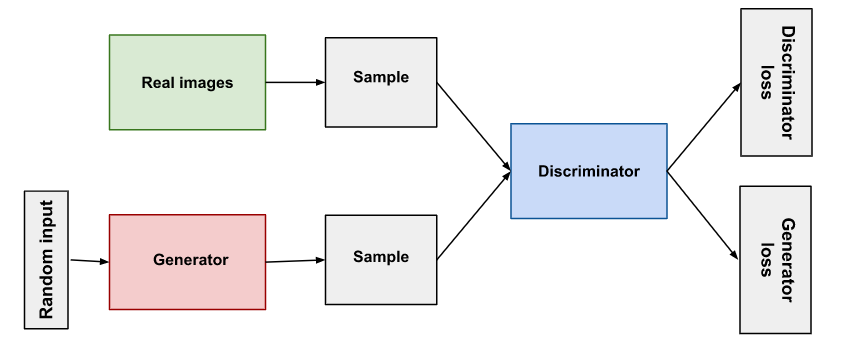
\includegraphics[width=\columnwidth]{images/gan.png}
    \caption{Both the generator and the discriminator are neural networks. The generator output is connected directly to the discriminator input. Through backpropagation, the discriminator's classification provides a signal to the generator which is used to update its weights.}
    \label{fig:gan.png}
\end{figure}
    Generative adversarial network, proposed by \citeauthor{goodfellow2014gan} \cite{goodfellow2014gan} belongs to the set of generative models. Figure \ref{fig:gan.png} shows the basic framework of GAN. This network has two parts:
\begin{itemize}
  \item The generator learns to generate plausible data. The generated instances become negative training examples for the discriminator.
  \item The discriminator learns to distinguish the generator's fake data from real data. The discriminator penalizes the generator for producing implausible results.
\end{itemize}

    When training begins, the generator produces obviously fake data, and the discriminator quickly learns to tell that it's fake. The discriminator in a GAN is simply a classifier. It tries to distinguish real data from the data created by the generator.The discriminator's training data comes from two sources:
\begin{itemize}
  \item \textbf{Real data} instances, such as real pictures of people. The discriminator uses these instances as positive examples during training.
  \item \textbf{Fake data} instances created by the generator. The discriminator uses these instances as negative examples during training.
\end{itemize}
 
 The generator tries to minimize the following function while the discriminator tries to maximize it:

\begin{equation}
    \mathbb{E}_{x}[\log(D(x))] + \mathbb{E}_z[\log(1-D(G(z)))]
\end{equation}
    In this function:
\begin{itemize}
        \item D(x) is the discriminator's estimate of the probability that real data instance x is real.
        \item \( \mathbb{E}_x\) is the expected value over all real data instances.
         \item G(z) is the generator's output when given noise z.
        \item D(G(z)) is the discriminator's estimate of the probability that a fake instance is real.
        \item \( \mathbb{E}_x\) is the expected value over all random inputs to the generator (in effect, the expected value over all generated fake instances G(z)).
        \item The formula derives from the cross-entropy between the real and generated distributions.
\end{itemize}
The generator can't directly affect the $ log(D(x)) $ term in the function, so for the generator, minimizing the loss is equivalent to minimizing $ log(1 - D(G(z))) $.        
        
\section{SeqGAN}

In this project, we have used the SeqGAN architecture by \citeauthor{yu2016seqgan} \cite{yu2016seqgan}. It generates text contents similar to the true data by using generative adversarial network, which is tweet from social bots in our case. 

Thre are two main reasons for using this architecture instead of the baseline GAN architecture. First, GAN is designed for generating real-valued, continuous data but has difficulties in directly generating sequence of discrete tokens. Secondly, GAN can only give the score/loss for an entire sequence when it has been generated. It is important to decide the is a generated sequence good enough for now or we need to keep generating.Thus, GAN is not efficient for partial-sequence scoring. 

\subsection{Overall Framework}

Figure \ref{fig:seqgan} illustrates the basic framework of SeqGAN. The generative model is treated as an agent of reinforcement learning, the state is the generated tokens so far and the action is the next token to be generated. The discriminator $ D $ is to evaluate the sequence and feedback the score/loss to guide the generative model. Monte Carlo search is employed to approximate the state-action value.

The sequence generation problem can be formalized as the following. Given a dataset of real-world structured sequences, train a $ \theta $-parameterized generative model $ G_{\theta} $ to produce a sequence $ Y_{1:T} = (y_1, ..., y_t,...,y_T), y_t \in \mathcal{Y} $, where $ \mathcal{Y} $ is the vocabulary of candidate tokens. In timestep $ t $, the state $ s $ is the current produced tokens $ (y_1,...,y_{t_1}) $ and the action $ a $ is the next token $ y_t $ to select. 

\begin{figure}
	\centering
	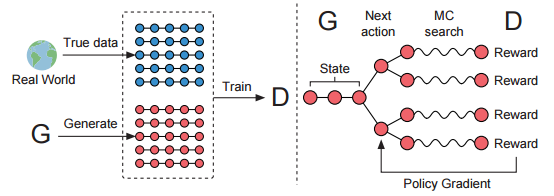
\includegraphics[width=\columnwidth]{seqgan.png}
	\caption{The illustration of SeqGAN. The left part shows that the Discriminator $ D $ is trained over the real data and the generated fake data by generator $ G $. The right part shows that the generator $ G $ is trained by policy gradient where the final reward is provided by discriminator $ D $ and is passed back to the intermediate action value via Monte Carlo search.\cite{yu2016seqgan}}	
	\label{fig:seqgan}
\end{figure}

The objective of the generator model $ G_{\theta}(y_t|Y_{1:t-1}) $ is to generate a sequence from the start state $ s_0 $ to maximize its expected end reward:

\begin{equation} \label{weight}
	J_{\theta} = \mathbb{E}[R_T|s_0, \theta] = \sum_{y_1 \in \mathcal{Y}} G_{\theta}(y_t|s_0) \cdot Q^{G_{\theta}}_{D_\phi}(s_0,y_1)
\end{equation}

where $ R_T $ is the reward for a complete sequence. The reward is from the $ \phi $-parameterized discriminator $ D_{\phi} $. $ Q^{G_{\theta}}_{D_\phi}(s_0,y_1) $ is the action-value function of a sequence, i.e. the expected accumulative reward starting from state $ s $, taking action $ a $, and then following policy $ G_{\theta} $. Note that, the reward is considered as the estimated probability of being real by the Discriminator. This objective function implies that starting from a given initial state, the goal of the Generator is to generate a sequence which would make the discriminator consider it is real.

\subsection{The Generative Model for Sequences}

The SeqGAN use recurrent neural networks (RNNs) (\citeauthor{hochreiter1997long} \cite{hochreiter1997long}) as the generative model. An RNN maps the input embedding representations $ \bm{x_1},..., \bm{x_T} $ of the sequence $ x_1,..., x_T $ into a sequence of hidden states $ \bm{h_1},...,\bm{h_T} $ by using the update function $ g $ recursively.

\begin{equation}\label{eq3}
	\bm{h_T} = g(\bm{h_{t-1}}, \bm{x_T})
\end{equation}

Moreover, a softmax output layer maps the hidden states into the output token distribution. In our implementation, we use seq2seq model by \citeauthor{luong17} \cite{luong17} as our RNN. Figure \ref{fig:seq2seq} shows the basic architecture of a seq2seq model. 

\begin{figure}
	\centering
	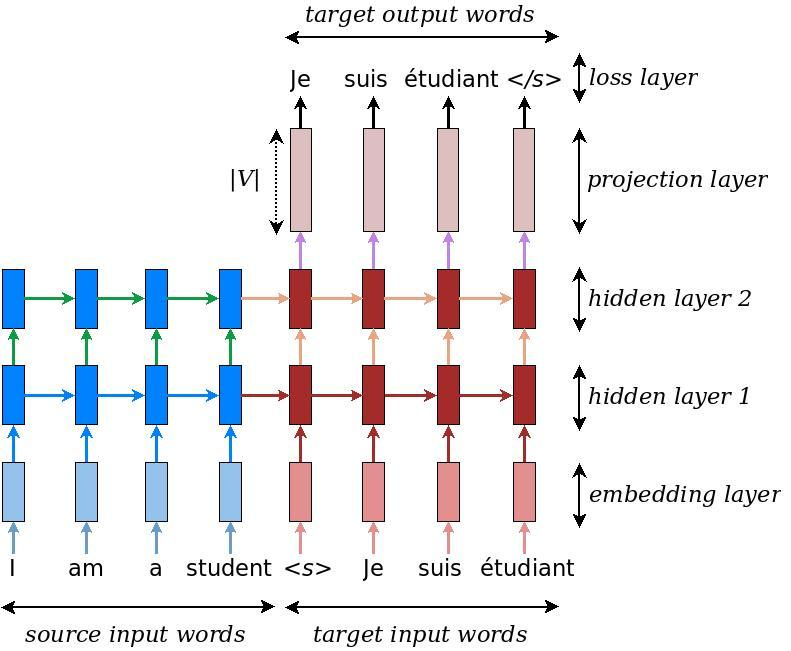
\includegraphics[width=\columnwidth]{seq2seq.jpg}
	\caption{The illustration of Seq2Seq model by \cite{luong17}. In our case, in order to generate random text. The source input words would be random cell states and hidden states. The projection layer corresponds to the softmax output layer which maps our hidden states into the output token distribution.}	
	\label{fig:seq2seq}
\end{figure}

\subsection{The Discriminative Model for Sequences}

In this project, CNN is chosen as our discriminator as CNN has recently been shown of great effectiveness in text (token sequence classification). The optimization target is to minimize the cross entropy between the ground truth label and the predicted probability. Figure \ref{fig:cnn} demonstrate a simple example of a CNN classifier on text. 

\begin{figure}
	\centering
	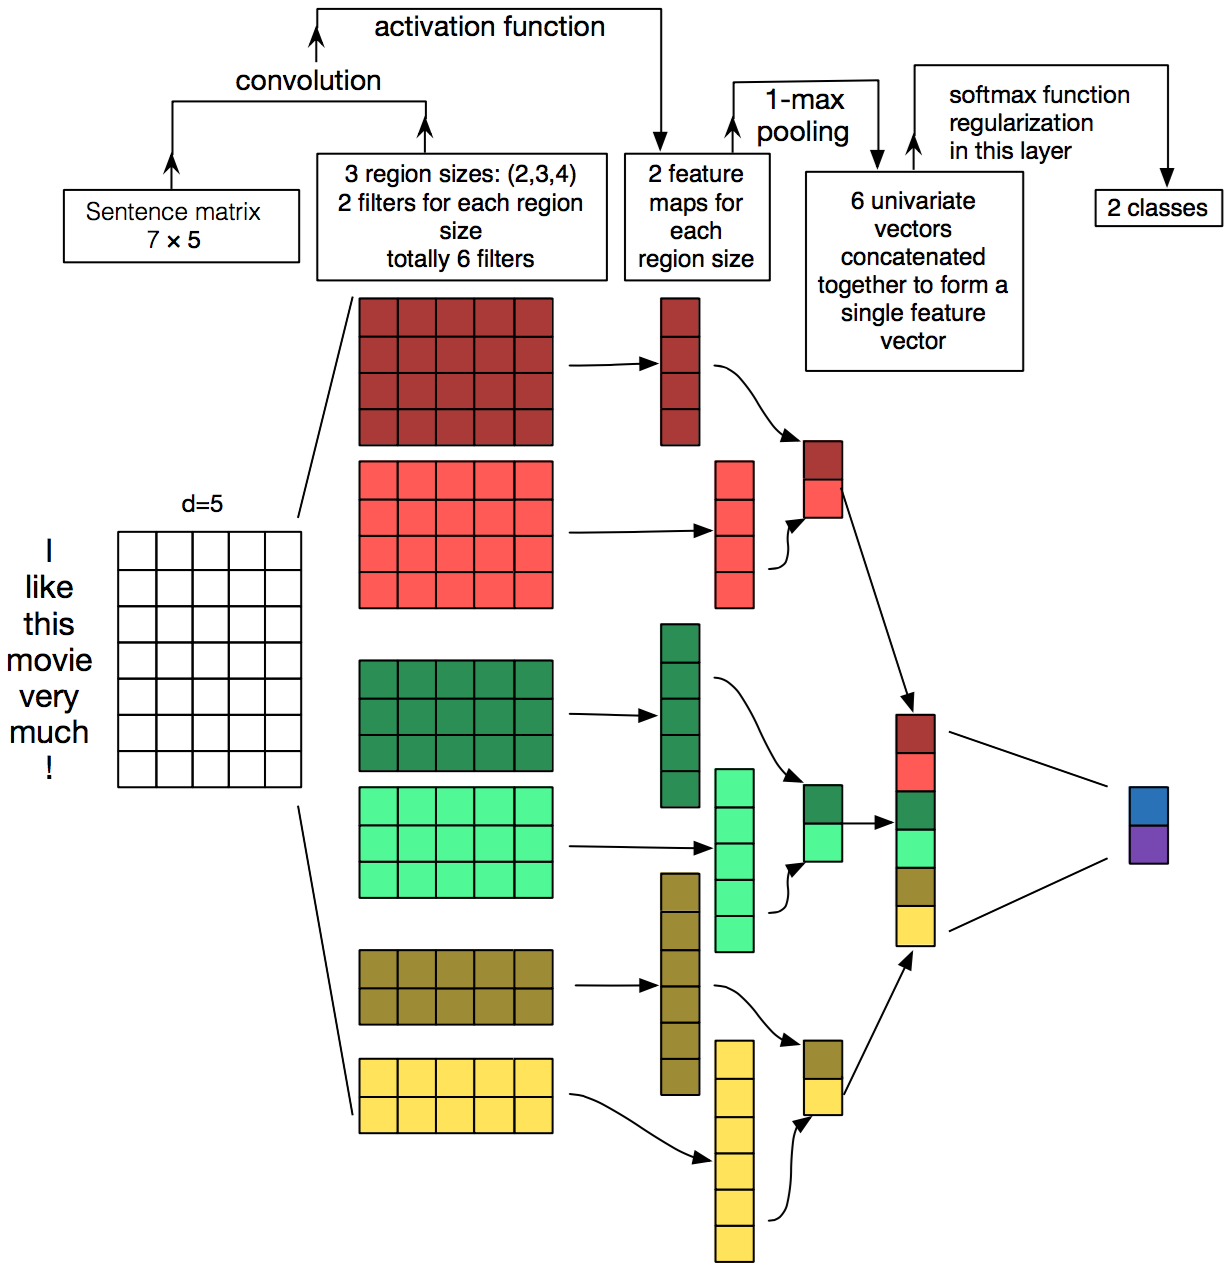
\includegraphics[width=\columnwidth]{cnn.png}
	\caption{This is a example of how a CNN classifier work. We concatenate the token embedding vector into a 2 dimensional matrix. Then we perform convolution by various number of kernels with different window size over the matrix to extract different features. After that, we apply a max-over-time pooling operation over the feature map. Finally, a fully connected layer with sigmoid activation is used to output the probability that the input sequence is real.}	
	\label{fig:cnn}
\end{figure}


\section{Related Work}

Following the limitation of GAN, pertinent to the generation of discrete data, such as words, various methods have been proposed to generate a sequence. One of the most popular methods is of the Recurrent Neural Network (RNN), which is used to produce a sequence of tokens and maximize their likelihood given a context \cite{bahdanau2014neural} \cite{sutskever2014sequence} . 

\citeauthor{kawthekarevaluating} \cite{kawthekarevaluating} used the cross-entropy loss function to train the model using Maximum Likelihood Estimation (MLE). The process starts by feeding in words of a given sentence at each epoch and the expected output for each step becomes serves as the next word in the sentence. 

\citeauthor{yu2016seqgan} and \cite{yu2016seqgan} used a similar approach. MLE was used to  train the generator in the pre-train stage, while the cross-entropy loss was used to train the discriminator in the pre-train stage. The benefit that the cross-entropy loss function provides is that as the difference between the true label and the predicted label (in terms of probability) increases, the discriminator loss increases as well. In this way, an objective for the loss function can be designed, which can minimize the cross-entropy loss.
\begin{equation}\label{eq_cross}
\min_{\phi}- \mathbb{E}_{Y \sim pdata}[log D_\phi(Y)]-\mathbb{E}_{Y \sim G_\theta}[log(1-D_\phi(Y))]
\end{equation}

A number of researchers have worked on devising a reward function for the generator. The challenge here is that during the early stages of generation, a sequence of words will almost always be treated as a bad sequence, discrediting the information in the sequence. For this reason, step-wise reward algorithms have been proposed. \citeauthor{tuan2018improving} \cite{tuan2018improving} used the step-wise GAN (stepGAN) to reward the generator after every step. A single epoch is divided into multiple steps, and evaluation is done based on results / word sequence generated in the particular step with the step input. 

A similar approach is carried out in the Monte Carlo Tree Search (MCTS) algorithm. MCTS generate random roll outs, and a reward is generated for each word \cite{Browne12asurvey, kawthekarevaluating}, as shown in figure \ref{fig:MCTS}. Word probabilities at the end of a state are back-propagated to the selection stage, and the word with the highest probability is selected as the next word in the sequence. 

\begin{figure}
	\centering
	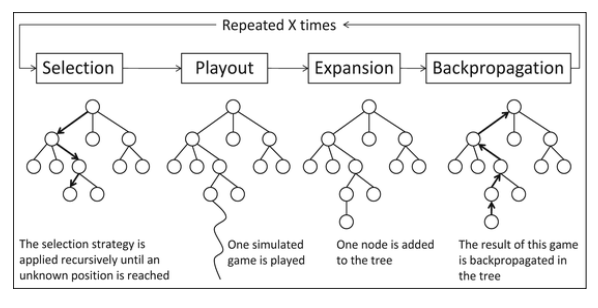
\includegraphics[width=\columnwidth]{images/figure_3.png}
	\caption{MCTS working algorithm}	
	\label{fig:MCTS}
\end{figure}



\section{Experiment}
\subsection{Experiment Design}
    Our study has used already labelled data, available online from the Social Honeypot Dataset\footnotemark \  by \citeauthor{Lee2011SevenMW} \cite{Lee2011SevenMW}. The dataset comprised of more than 3 million tweets from legitimate (real) users and approximately 2 million bot tweets. The real tweet data was reduced to approximately 100k tweets for computational ease.

    The Experiment was conducted in two stages; Pre-Training and Training. For the Pre-Training phase, an  vocab file was created for the tweets using the One-Hot Vector method. This allowed both the discriminator and generator to learn English words and produce similar words or combination of words and not just garbage text. 
    \footnotetext{http://infolab.tamu.edu/data/}

\subsection{Training Algorithm}

\begin{algorithm}\label{alg1}
\caption{Sequence Generative Adversarial Nets}
\SetAlgoLined
\textbf{Require} : generator policy G\textsubscript{$\theta$};
{rollout policy} G\textsubscript{$\beta$}; discriminator 
{D\textsubscript{$\phi$}}; a sequence dataset 
{$S$} = $\left\{ X\textsubscript{1:T}\right\}$\\
Initialize G\textsubscript{$\theta$},G\textsubscript
{$\theta$}
with random weights $\theta$,$\phi$.\\
Pre-Train G\textsubscript{$\theta$} using MLE on $S$\\
$\beta$ $\leftarrow$ $\theta$\\
Generate negative samples using G\textsubscript{$\theta$} for training D\textsubscript{$\phi$}\\
Pre-train D\textsubscript{$\phi$} via minimizing cross entropy\\
\textbf{repeat}\\
\For{g\_steps}
{Generate a sequence Y$_{1:T}$ = (y$_1$,...,y$_T$) $\sim$ 
G$_\theta$\\
\For{t in 1:T}
{Compute Q($a=y$\textsubscript{$t$};
 $s=Y$\textsubscript{$1:t-1$}) }
Update Generator parameters via Policy Gradient 
}
\For{d\_steps}
{Use current G$_\theta$ to generate negative samples and combine with the given positive samples $S$\\
Train Discriminator D$_\phi$ for k epochs by Eq. \eqref{eq_cross}
}
$\beta$ $\leftarrow$ $\theta$\\
\textbf{until} SeqGAN converges\\ 
\end{algorithm}

Algorithm \ref{alg1} shows full details about the SeqGAN, referenced from \cite{yu2016seqgan}. At the beginning of the training, we use the Maximum Likelihood Estimation (MLE) to pre-train the Generator G$_\phi$ on the dataset $S$. After the pre-training the generator and the discriminator are trained alternatively. As the generator gets progressed on g-steps updates, the discriminator has to be trained periodically to be able to identify the real and fake samples effectively.
When training the discriminator the positive samples are from the dataset and the negative samples are obtained from the generator. In order to maintain balance we use equal number of positive and negative samples to train the discriminator.
The reward function generates Intermediate Rewards, i.e Token wise rewards for partial sequences. Use of MCTS

\subsection{Results}
Initially, we pre-trained with the entire dataset, hoping to improve the efficiency during the adversarial training stage. However, this resulted in the generator learning the entire dataset and mimicking the input tweets rather than generating new sequences.

We then used $ 20\% $ dataset for the pre-training and $ 80\% $ for the adversarial training. This improved both the processing time and the discriminator ability to distinguish between real and generated-tweets, thus, improving the overall performance of the Generator also.

Figure \ref{fig:Results} presents the training results. It can be seen that during the initial epochs, the training losses for both the Generator and the Discriminator fluctuates considerably around 0.5 (the midpoint). This indicates  the learning battle between the Generator and the Discriminator, where each tries to outperform the other. After 120 epochs, both the Discriminator and Generator losses are closed to 0.5. This indicates a 50\% probability for a Discriminator to catch a fake, i.e. computer-generated tweet, while a 50\% probability for the Generator to fool the Discriminator and get labelled as a legitimate tweet. The Generator loss at the end of the training is still away from the ideal mark, because of the presence of rare and unknown words in the tweets, which are hard to learn for the Generator. 

\begin{figure}
	\centering
	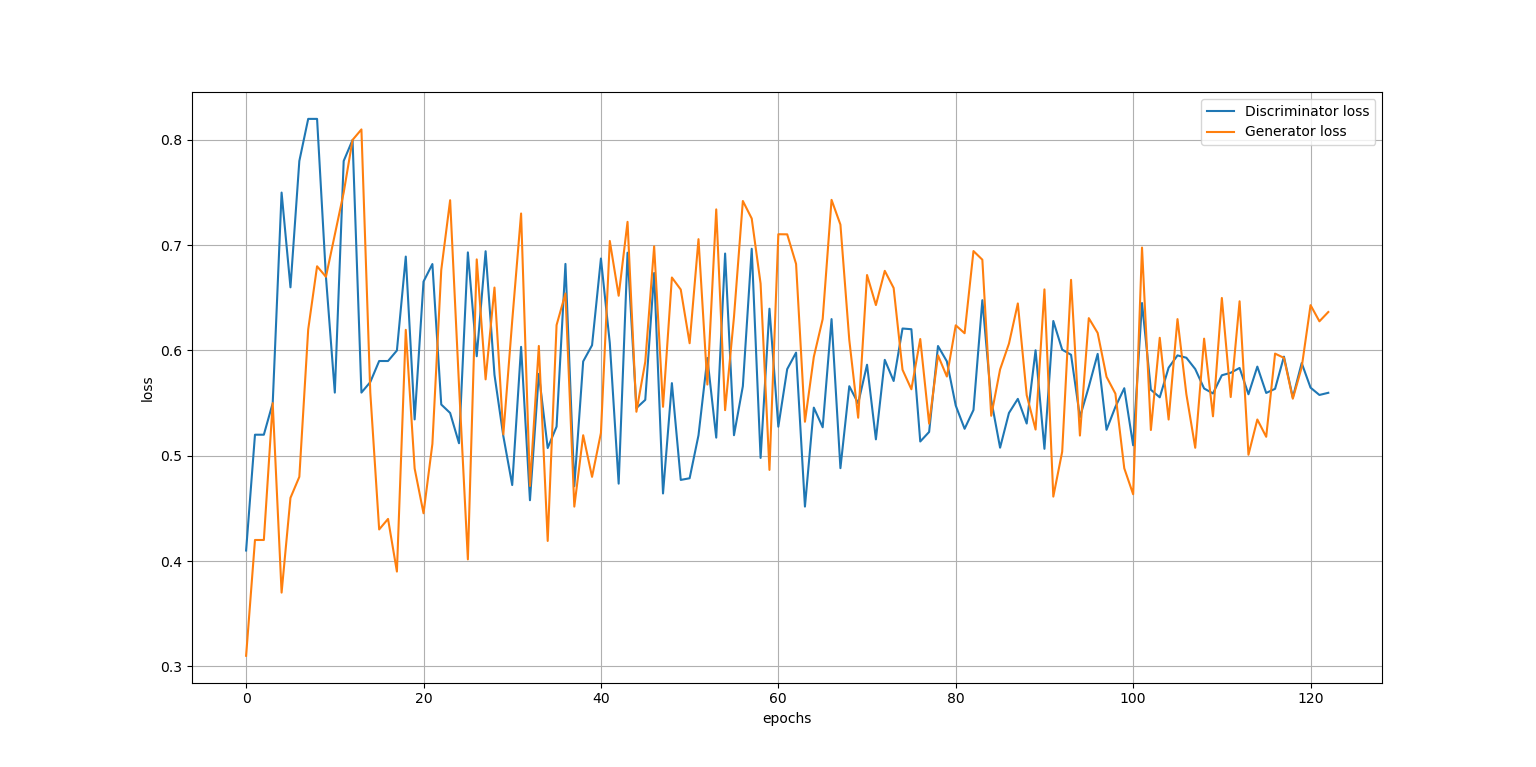
\includegraphics[width=\columnwidth]{images/Figure_6.png}
	\caption{Training loss curves for Discriminator and Generator}	
	\label{fig:Results}
\end{figure}

Some of the sample tweets generated by the trained generator are presented in Table \ref{tab:gen_samples}. Though, some tweets may not make a complete sense logically to humans, but the majority of the tweets generated were grammatically correct, and it would be very hard for a bot-detector to classify them as computer-generated tweets. This further stresses on the strength of the adversarial network to learn word sequencing, which more often than not also offers a semantically correct presentation. 

\begin{table}[h]
    \centering
     \caption{Tweets generated by the Generator after 100 epochs}
    \begin{tabular}{|p{3cm}|p{4.5cm}|}
    Generated Tweets &   Related Real Tweets \\
    \hline 
   Ending slavery, Betty White House. & One group wanted to abolish slavery while other was talking about states rights \& "property". \\
    
    Put with Donald Trump for the future leaks in Philadelphia. & Donald Trump just fired four in one fell swoop in The Apprentice USA! Makes Suralan look meek and mild! \\
    
    We did n’t have transgender bathroom ever to soda after massive much & Internet Radio kicks off Transgender Awareness Week. \\
   \end{tabular}
   \label{tab:gen_samples}
\end{table}




\section{Conclusion}
We were able to create an Adversarial Network that can learn from text and create new text sequences, which adhere to the English grammar parameters. One of the limitations of the network is that the current algorithm is dependent on the initial parameters. If we pre-train with a large (actual) dataset, the generator memorizes everything and creates the same texts rather than using the word-embedding technique. This was taken care by dividing the tweet dataset into proportionate chunks for pre-training and adversarial training. 

Furthermore, in the final epoch, the Generator still produces "UNK" labels for the unknown/ rare words. One technique to remove this is of manually replacing all "UNK" labels with related words using the embedded maps. A selection algorithm can be used to provide this functionality.



\bibliographystyle{plainnat}
\small
\bibliography{references}

\section{Acknowledgements}
We sincerely thank Prof. Dr. Stefan Evert, Dr. Vincent Christlein, Anguelos Nicolaou, Ronak Vijaypal Kosti, and Prof. Dr.-Ing. Andreas Maier for many helpful discussions and comments on the project and the manuscript.



\end{document}

